\chapter{Boltzmann Machines}
\label{sec:rbm}
The following chapter gives an introduction to Boltzmann machines and their applications to the classical 
simulation of quantum computing.

An overview of the architecture and mathematical properties of Boltzmann machines are given in the first section. The restricted Boltzmann machine is motivated as a special kind of Boltzmann machine with useful mathematical properties in the second part of this chapter. Afterward, the concepts of Gibbs sampling and supervised learning are explained.
In the last section, a constructive approach on how restricted Boltzmann machines 
can be applied to the classical simulation of quantum computing is given.

The introduction to Boltzmann machines and restricted Boltzmann machines as well as the introduction 
to Gibbs sampling are based on \cite{montufar2018restricted} and 
\cite{fischer2012introduction} which provide a more throughout introduction 
into the topic. The work of J\'{o}nsson, Bauer and Carleo \cite{jnsson2018neuralnetwork} is the 
foundation of the last section of this chapter.

\section{Characteristics}
\label{sec:gbm}
The concept of the Boltzmann machine has first been proposed in the 1980s as a
model for parallel distributed computing \cite{hinton1983analyzing}. Boltzmann machines are physically inspired by the Ising Spin model and can be interpreted as energy-based recurrent neural networks representing probability distributions
over vectors $\bm{d}_i \in \{0,1\}^n$ \cite{ackley1985learning}.

A Boltzmann machine is a network of stochastic units (or neurons) $X=V \cup H$ which are segmented into
\textit{visible} neurons $V=\{v_1, \dots, v_n\}$ and \textit{hidden} neurons $H=\{h_1, \dots, h_m\}$.
The joint state of the visible neurons $\bm{v} = (v_1\dots v_n) \in \{0,1\}^n$ represents n-dimensional data
points $\bm{d}_i \in \{0,1\}^n$. The hidden neurons increase the expressiveness of the Boltzmann machine by acting as non-linear feature 
detectors to model dependencies between the visible neurons \cite{hinton2010boltzmann}.

The neurons are 
connected to each other by weighted links $W_{ij}$ and poss biases $a_i$ (visible) or $b_i$ (hidden), respectively. In 
general, the neurons of a Boltzmann machine can be fully connected. A graphical representation of a fully connected Boltzmann machine is shown in figure~\ref{fig:boltzmannMachine}.

\begin{figure}[H]
    \centering
    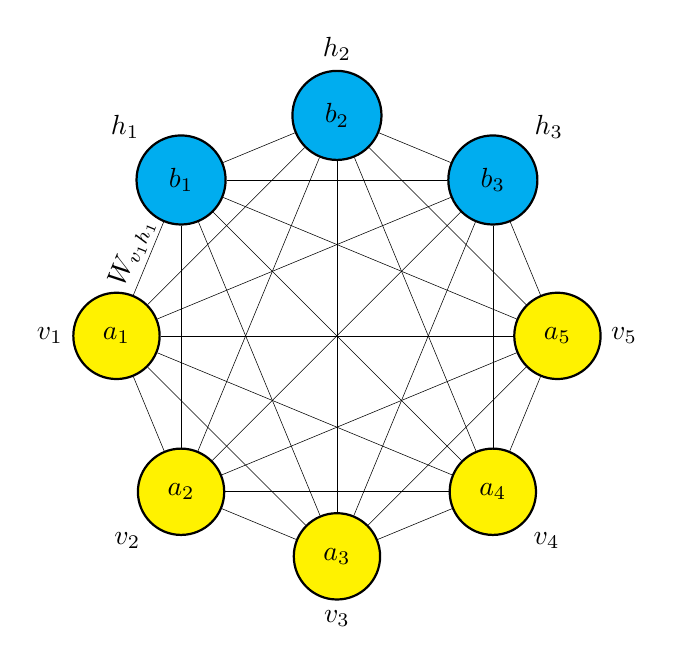
\begin{tikzpicture}[transform shape,line width=0.2pt]
        \foreach \x in {1,...,8}{%
            \pgfmathparse{(\x-1)*45+floor(\x/9)*22.5}
            \node[label={\pgfmathresult:\ifnum\x=1 $v_5$\else\ifnum\x=2 $h_3$\else\ifnum\x=3 $h_2$\else\ifnum\x=4 $h_1$\else\ifnum\x=5 $v_1$\else\ifnum\x=6 $v_2$\else\ifnum\x=7 $v_3$\else\ifnum\x=8 $v_4$\fi\fi\fi\fi\fi\fi\fi\fi},draw,circle,inner sep=0.25cm,fill={\ifnum\x=1 yellow\else\ifnum\x<5 cyan\else yellow\fi\fi}] (N-\x) at (\pgfmathresult:2.8cm) [thick] {\ifnum\x=1 $a_5$\else\ifnum\x=2 $b_3$\else\ifnum\x=3 $b_2$\else\ifnum\x=4 $b_1$\else\ifnum\x=5 $a_1$\else\ifnum\x=6 $a_2$\else\ifnum\x=7 $a_3$\else\ifnum\x=8 $a_4$\fi\fi\fi\fi\fi\fi\fi\fi};
        }
        \foreach \x [count=\xi from 1] in {2,...,8}{%
            \foreach \y in {\x,...,8}{%
                \ifnum\y=5 \else\ifnum\xi=5 \else \path (N-\xi) edge[-] (N-\y)\fi\fi;
            }
        }
        \draw (N-5) -- (N-1) node [] (E-1) {};
        \draw (N-5) -- (N-2) node [] (E-2) {};
        \draw (N-5) -- (N-3) node [] (E-3) {};
        \draw (N-5) -- (N-4) node [midway,above=-0.06cm,sloped] (E-4) {$W_{v_{1}h_{1}}$};
        \draw (N-5) -- (N-6) node [] (E-5) {}; 
        \draw (N-5) -- (N-7) node [] (E-6) {};
        \draw (N-5) -- (N-8) node [] (E-7) {};
    \end{tikzpicture}
    \caption[Fully Connected Boltzmann Machine]{Graphical representation of a fully connected Boltzmann machine with 5 visible neurons (yellow) $v_1$ to $v_5$
    and 3 hidden neurons (blue) $h_1$ to $h_3$. Each neuron posses a bias
    $a_1$ to $a_5$ and $b_1$ to $b_3$ respectively. The connection weight between two neurons $i$ and $j$
    is given by $W_{ij}$.}
    \label{fig:boltzmannMachine}
\end{figure}

Each configuration $\bm{c}=(v_1,\dots,v_n,h_1,\dots,h_m)$ of neuron states
of the Boltzmann machine is associated with an energy $E(\bm{c})$ value,
which is defined by the parameters $\mathcal{W}$ consisting of the weights and 
biases $\mathcal{W} = \{a_i, b_j, W_{ij}\}$:

\begin{equation}
  E(\bm{c};\mathcal{W}) = - \sum_{v_i \in V} a_{i}v_{i} - \sum_{h_i \in H} b_{i}h_{i} - \sum_{x_i,x_j \in X} W_{x_i,x_j}x_{i}x_{j}.
\end{equation}

When sampling configurations from the Boltzmann machine (discussed in more detail in section~\ref{sec:gibbsSampling}), the 
Boltzmann machine prefers low energy states over states with high energies. The \textit{stationary probability}
of a configuration $\bm{c}$ with energy $E(\bm{c};\mathcal{W})$ is given by the so-called \textit{Gibbs-Boltzmann distribution} \cite{gibbs_2010}

\begin{equation}
   p(\bm{c};\mathcal{W}) = \frac{\mathrm{e}^{-E(\bm{c};\mathcal{W})}}{Z(\mathcal{W})},
\end{equation}

where $Z(\mathcal{W})$ is the normalizing partition function 

\begin{equation}
   Z(\mathcal{W}) = \sum_{\bm{c}\prime\in C} \mathrm{e}^{-E(\bm{c}\prime;\mathcal{W})}.
\end{equation}

In a training phase (discussed in section~\ref{sec:learning} ), the parameters of the Boltzmann machine can be adapted in such a way that 
the marginal probability distribution $p(\bm{v}; \mathcal{W})$ of the visible neurons

\begin{equation}
    \label{eq:gbm}
   p(\bm{v};\mathcal{W}) = \sum_{\bm{h}_k \in \{0,1\}^m} p(\bm{v},\bm{h}_k;\mathcal{W}),
\end{equation}

which traces out the hidden unit 
states by summing over all possible configurations of them, resembles the probability 
distribution of data points $\bm{d}_i$ in a training set $D=\{\bm{d}_1,\dots,\bm{d}_l\}$.

For a fully connected Boltzmann machine, this representation consists of an exponential number of summands and cannot be calculated efficiently. So-called \textit{restricted Boltzmann machines}
have a specific architecture with a restricted connectivity, which allows the efficient calculation of the marginal probability.

\section{Restricted Boltzmann Machines}
\label{sec:rbms}
The \gls{rbm} is a type of Boltzmann machine with 
a specific architecture and properties \cite{smolensky1986information}. Since their invention \gls{rbm}s have been applied to a variety 
of machine learning tasks. They played a 
key role in the development of deep learning architectures as building blocks of so-called 
\textit{Deep Belief networks} \cite{bengio2009learning, hinton2006fast}.
\gls{rbm}s are the kind of Boltzmann machines which are used in this study of the simulation 
of quantum circuits.

In its restricted form, the neurons of the Boltzmann machine are separated into two layers;
one being the visible layer containing the visible neurons $v_i \in V$ and the other layer being the hidden layer containing the hidden neurons $h_j \in H$. Each neuron of the \gls{rbm} 
is only allowed to be connected to the neurons from the other layer. Intra-layer connections are not allowed. As a result, the graph of the \gls{rbm} is bipartite as shown in figure~\ref{fig:rbm}. 

\begin{figure}[H]
    \centering
    \begin{tikzpicture}[transform shape,line width=0.2pt]
    
        \node (v1)[neuron, fill=yellow] at (0, 0) {$a_1$};
        \node (v2)[neuron, fill=yellow] at (2, 0) {$a_2$};
        \node (v3)[neuron, fill=yellow] at (4, 0) {$a_3$};
        \node (v4)[neuron, fill=yellow] at (6, 0) {$a_4$};
        \node[below=0.1cm of v1] (bv1) {$v_1$};
        \node[below=0.1cm of v2] (bv2) {$v_2$};
        \node[below=0.1cm of v3] (bv3) {$v_3$};
        \node[below=0.1cm of v4] (bv4) {$v_4$};
    
        \node (h1)[neuron, fill=cyan] at (1, 2) {$b_1$};
        \node (h2)[neuron, fill=cyan] at (3, 2) {$b_2$};
        \node (h3)[neuron, fill=cyan] at (5, 2) {$b_3$};
        \node[above=0.1cm of h1] (bh1) {$h_1$};
        \node[above=0.1cm of h2] (bh2) {$h_2$};
        \node[above=0.1cm of h3] (bh3) {$h_3$};
    
        \draw (v1) -- (h1) node [midway,above=-0.06cm,sloped] {$W_{v_1h_1}$};
        \draw (v1) -- (h2) node [midway,above=-0.06cm,sloped] {};
        \draw (v1) -- (h3) node [midway,above=-0.06cm,sloped] {};
    
        \draw (v2) -- (h1) node [midway,above=-0.06cm,sloped] {};
        \draw (v2) -- (h2) node [midway,above=-0.06cm,sloped] {};
        \draw (v2) -- (h3) node [midway,above=-0.06cm,sloped] {};
    
        \draw (v3) -- (h1) node [midway,above=-0.06cm,sloped] {};
        \draw (v3) -- (h2) node [midway,above=-0.06cm,sloped] {};
        \draw (v3) -- (h3) node [midway,above=-0.06cm,sloped] {};
    
        \draw (v4) -- (h1) node [midway,above=-0.06cm,sloped] {};
        \draw (v4) -- (h2) node [midway,above=-0.06cm,sloped] {};
        \draw (v4) -- (h3) node [midway,above=-0.06cm,sloped] {};
    \end{tikzpicture}
    \caption[Restricted Boltzmann Machine]{Graphical representation of a \gls{rbm} with 5 visible neurons and 3 hidden ones. 
    There are only connections between the two layers and no connection between two neurons 
    from the same layer.}
    \label{fig:rbm}
\end{figure}

The marginal probability $p(\bm{v};\mathcal{W})$ of the visible neuron states in a \gls{rbm} has the form:

\begin{align}
   p(\bm{v};\mathcal{W}) &= \sum_{\bm{h}_k \in \{0,1\}^m} p(\bm{v},\bm{h}_k;\mathcal{W})\\
   &= \frac{1}{Z(\mathcal{W})}\sum_{\bm{h}_k \in \{0,1\}^m} \mathrm{e}^{-E(\bm{v}, \bm{h}_k;\mathcal{W})}\\
   &= \frac{1}{Z(\mathcal{W})}\sum_{h_1\in \{0,1\}}\dots\sum_{h_m \in \{0,1\}}\mathrm{e}^{\sum_{v_i}b_iv_i}\prod_{j=1}^m\mathrm{e}^{h_j(b_j + \sum_{i=1}^nW_{ij}v_i)}\\
   &= \frac{\mathrm{e}^{\sum_{v_i}b_iv_i}}{Z(\mathcal{W})}\sum_{h_1 \in \{0,1\}}\mathrm{e}^{h_1(b_1 + \sum_{i=1}^nW_{i1}v_i)}\dots\sum_{h_m \in \{0,1\}}\mathrm{e}^{h_m(b_m + \sum_{i=1}^nW_{im}v_i)}\\
   &= \frac{\mathrm{e}^{\sum_{v_i}b_iv_i}}{Z(\mathcal{W})}\prod_{i=1}^m\sum_{h_i \in \{0,1\}}\mathrm{e}^{h_i(b_i + \sum_{i=1}^nW_{ij}v_i)}\\
   \label{eq:rbm}
   &= \frac{\mathrm{e}^{\sum_{v_i}b_iv_i}}{Z(\mathcal{W})}\prod_{i=1}^m(1+\mathrm{e}^{b_i + \sum_{i=1}^nW_{ij}v_i}).
\end{align}

This quantity consists of only a polynomial number of terms in the number of hidden units of the \gls{rbm}. Consequently, it can be calculated efficiently. This makes the \gls{rbm} a compact representation of a probability distribution over vectors $\bm{d}_i \in D$ inferred from a dataset $D$.

Even though the \gls{rbm} has a limited connectivity between its units, it is a universal function approximator \cite{le2008representational}.
It can model any distribution over $\{0,1\}^m$ arbitrary well with $m$ visible and $k+1$ hidden units, where 
$k$ denotes the cardinality of the support set of the target distribution. This is the number of input elements
from $\{0,1\}^m$ that have a non-zero probability of being observed. This also implies a worst-case 
exponential number of hidden units for distributions with an extensive support set \cite{le2008representational}. Fewer units can be sufficient depending on the patterns in the support set \cite{montufar2011refinements}.

\section{Gibbs Sampling}
\label{sec:gibbsSampling}

Boltzmann machines are generative models that represent probability distributions over their configurations. This means that it is possible to draw configurations from a Boltzmann machine
according to their (marginal) probabilities given in equations~\ref{eq:gbm} and \ref{eq:rbm}.

Although it is required to calculate $Z(\mathcal{W})$ for the exact probabilities of each configuration,
it is not necessary to calculate the energies for all $2^{n+m}$ possible configurations of 
a Boltzmann machine to draw samples from it.

Instead, Boltzmann machines can be seen as \textit{Markov chains} with a stationary probability
distribution. With a stochastic process called \textit{Gibbs sampling} the samples can be drawn efficiently according to this stationary distribution for \gls{rbm}s.

Gibbs sampling belongs to the class of so-called \textit{Metropolis-Hastings} algorithms. By that, it is 
a \textit{\gls{mcmc}} algorithm \cite{hastings1970monte}. It is a simple algorithm to produce samples from the joint probability distribution of multiple random variables like neuron state configurations
of a Boltzmann machine, which can be considered as a Markov chain.

A Markov chain is a discrete stochastic process of configurations of random variables $C=\{\bm{c}^{(t)}\}$
at time steps $t=1, \dots, T$ which take values in a set $\Omega$ (for Boltzmann machines 
$\Omega=\{0,1\}^{m+n}$) and for which for all time steps $t$ and for all configurations 
$\bm{c}_j, \bm{c}_i, \bm{c}_{i-1}, \dots, \bm{c}_0 \in \Omega$ the \textit{Markov property}

\begin{align}
    p_{ij}^{(t)} &:= P(\bm{c}^{(t+1)} = \bm{c}_j \mid \bm{c}^{(t)} = \bm{c}_i, \dots, \bm{c}^{(0)} = \bm{c}_0) \\
                 & = P(\bm{c}^{(t+1)} = \bm{c}_j \mid \bm{c}^{(t)} = \bm{c}_i) 
\end{align}

holds. This means that the next state of the system only depends on the current state and not on the system's history. A Markov chain can be represented as a (finite) graph, as shown in figure~\ref{fig:markov}.

\begin{figure}[H]
    \centering
    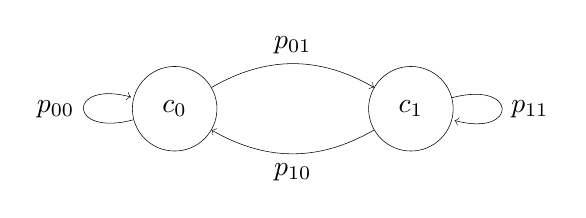
\begin{tikzpicture}[transform shape,line width=0.2pt]
    
        \node [draw,circle,inner sep=0.25cm] (s0) at (0,0) {$c_0$};
        \node [draw,circle,inner sep=0.25cm] (s1) at (3,0) {$c_1$};
    
        \path[->] (s0) edge[loop left]  node {$p_{00}$} (s0);
        \path[->] (s0) edge[bend left] node[above] {$p_{01}$} (s1);
        \path[->] (s1) edge[bend left] node[below] {$p_{10}$} (s0);
        \path[->] (s1) edge[loop right] node {$p_{11}$} (s1);
    
    \end{tikzpicture}
    \caption[Markov Chain with Two States]{A Markov chain with two states $c_0$ and $c_1$. The Markov chain is 
described by the $2 \times 2$ matrix $\bm{P}=\begin{pmatrix} p_{00} & p_{01} \\ p_{10} & p_{11} \end{pmatrix}$.}
    \label{fig:markov}
\end{figure}

In the case of Boltzmann machines, the transition probabilities $p_{ij}$ are time independent and 
given by the ratios of configuration probabilities. For \gls{rbm}s the transition probability $p_{ij}$ 
from configuration $c_i$ to $c_j$ is given by:

\begin{equation}
    p_{ij} = \frac{\mathrm{e}^{\sum_{v_i \in \bm{c_i}}b_iv_i}\prod_{i=1}^m(1+\mathrm{e}^{b_i + \sum_{i=1}^nW_{ij}v_i})}{\mathrm{e}^{\sum_{v_i \in \bm{c_j}}b_iv_i}\prod_{i=1}^m(1+\mathrm{e}^{b_i + \sum_{i=1}^nW_{ij}v_i})},
\end{equation}

which can be calculated efficiently as the $Z(\mathcal{W})$ terms from equation~\ref{eq:rbm} cancel out.

In each time step $t$ during the Gibbs sampling, the state of a single randomly chosen neuron of the \gls{rbm} is flipped
so that the configurations $\bm{c}^{(t)}$ and $\bm{c}^{(t+1)}$ only differ in the state of one neuron. With 
probability $p_{ij}$ configuration $\bm{c}_j$ is kept as the new configuration. With probability
$1-p_{ij}$ the Boltzmann machine will stay in its current configuration $\bm{c}_i$. This corresponds to a random walk on the Markov chain defined by the \gls{rbm} transition probabilities. The algorithm is given in 
algorithm~\ref{alg:gibbs}.

\begin{algorithm}[H]
    \caption{Gibbs Sampling}
    \begin{algorithmic}[1]
        \Require $bm(\bm{c})$: function returning the energy of a Boltzmann machine for configuration $\bm{c}$
        \Require T: time steps
        \State $t\gets 0$
        \State $\bm{c}^{(0)} \gets randomize(\{0,1\}^{m+n})$ (random initialization)
        \Repeat
            \State $r \gets random(m+n)$
            \State $E_i \gets bm(\bm{c}^{(t)})$
            \State $E_j \gets bm(\{c_1,\dots,\bar{c_r},\dots,c_{m+n}\})$
            \If{$random(1) < \frac{E_i}{E_j}$}
                \State $\bm{c}^{(t+1)} \gets \{c_1,\dots,\bar{c_r},\dots,c_{m+n}\}$
            \EndIf
            \State $t\gets t+1$
        \Until{$t=T$}
        \State \textbf{return} $\bm{c}^{(T)}$
    \end{algorithmic}
    \label{alg:gibbs}
\end{algorithm}

The Markov chain for configurations of a Boltzmann machine is known to converge to its so-called 
\textit{stationary distribution} $\pi$, that is

\begin{equation}
    \pi^T=\pi^T\bm{P}
\end{equation}

with $\bm{P} = (p_{ij})$ being the transition matrix of the Markov chain with the transition probabilities as its entries.
Once the Markov chain reaches its stationary distribution, all subsequent states will be distributed according to this distribution. Running Gibbs sampling for 
sufficiently many time steps $T$ will sample configurations according 
to the Gibbs-Boltzmann distribution given in equation~\ref{eq:rbm}.

Although Gibbs sampling is a simple algorithm, it is an important algorithm in the context of 
Boltzmann machines. Different versions of Gibbs sampling have been developed for \gls{rbm}s, like 
(persistent) contrastive divergence \cite{hinton2002training, tieleman2008training} or parallel tempering \cite{desjardins2010parallel}. In this study,
Gibbs sampling is used in its simplest version, as described in this chapter.
    
\section{Supervised Learning}
\label{sec:learning}
The probability distribution over vector spaces given by a Boltzmann machine can be trained to 
resemble the distribution of data points $\bm{d}_i$ in a dataset $D=\{\bm{d}_1,\dots,\bm{d}_d\}$. This can be done either in a \textit{unsupervised}
or in a \textit{supervised} manner.

In both cases the parameters $\mathcal{W} = \{a_i,b_j,W_{ij}\}$ of the Boltzmann machine are updated minimizing 
an objective function $O(\mathcal{W})$, which depends on the parameters of the Boltzmann machine and 
depicts the overlap of the current and the target distribution in an iterative process called \textit{gradient descent}.

Before the training phase, the Boltzmann machine is initialized with random parameters $\theta_i \in \mathcal{W}_0$ and a training set 
$D=\{\bm{d}_1,\dots,\bm{d}_d\}$ is given. In the case of supervised learning of Boltzmann machines, the training set consists of tuples of configurations and their corresponding target energy values $\bm{d}_i= (\bm{c}_i, t_i)$.

In the batch version of gradient descent the training set $D$ is 
split into subsets $D_1, \dots, D_l$, called \textit{batches}.

For each such batch $D_i$ the average negative log overlap $\langle L(\mathcal{W})\rangle$ for all $\bm{c}_j \in D_i$
is computed. Afterward, the gradients $\frac{\partial L}{\partial \delta_i}$ are calculated and the parameters updated into
the direction of the steepest descent:

\begin{equation}
    \label{eq:sgd}
    \theta_i = \theta_i - \alpha \frac{\partial L}{\partial \delta_i}
\end{equation}

with \textit{learning rate} $\alpha \ll 1$ to keep the step sizes moderate. The learning rate prevents step sizes, which are too big in steep 
areas of the objective function $L(\mathcal{W})$.
This process is repeated for a defined number of iterations to minimize the objective function $O(\mathcal{W})$.
A graphical representation of this process is shown in figure~\ref{fig:sgd}.

\begin{figure}[H]
  \centering
  \includegraphics[width=0.8\textwidth]{figures/gradient_descent}
  \caption[Gradient Descent]{Iterations of a gradient descent method. At each iteration the randomly initialized parameters are updated in 
   direction of the steepest descent of the function to be optimized. After enough iterations a minimum of the function is reached.}
  \label{fig:sgd} 
\end{figure}
 
The simple update rule in \ref{eq:sgd} has several drawbacks, however. First, The gradient and the step size become smaller as closer the function approaches its minimum, leading to only small improvements and many steps necessary.
Second, the function's shape will usually have (many) local minima, which should be avoided.
Several variants of gradient descent have been developed to overcome these issues \cite{ruder2016overview}.
Two of these methods are \textit{AdaMax} \cite{ruder2016overview} and \textit{\gls{sr}} \cite{sorella1998green}.

\subsection{AdaMax}
AdaMax is a special version 
of \textit{Adam} \cite{kingma2014adam}.It combines the advantages of AdaGrad \cite{duchi2011adaptive} and RMSProp \cite{bengio2015rmsprop},
two other popular gradient descent methods. AdaMax is computationally efficient, has little
memory requirements, and proves to be well suited for problems with much noise and sparse gradients.

Instead of using the raw gradient, the algorithm updates exponential moving averages of the gradient ($\bm{m}_t$) and the squared gradient
($\bm{v}_t$) to include more information about the shape of the error function into the parameter updates. The hyper-parameters $\beta_1, \beta_2 \in [0, 1)$ control the exponential decay rates of these moving
averages. The moving averages themselves are estimates of the 1st moment (the mean) and the
2nd raw moment of the gradient. The update rule for the parameters $\theta_{i} \in \mathcal{W}$ for AdaMax are summarized in 
algorithm~\ref{alg:adamax}.

\begin{algorithm}
    \caption{AdaMax}
    \begin{algorithmic}[1]
        \Require $\alpha$: step size
        \Require $\beta_1, \beta_2 \in [0,1)$: Exponential decay rates
        \Require $f(\mathcal{W})$: Stochastic objective function
        \Require $\mathcal{W}_0$: Initial parameter vector
        \State $\bm{m}_0 \gets \bm{0}$ (Initialize $1^{st}$ moment vector)
        \State $\bm{u}_0 \gets \bm{0}$ (Initialize the exponential weighted infinity norm)
        \State $t \gets 0$ (Initialize time step)
        \While {$\mathcal{W}_t$ not converged}
            \State $t\gets t+1$
            \State $\bm{g}_t \gets \nabla_{\mathcal{W}}f_t(\mathcal{W}_{t-1})$ (Get gradients w.r.t. objective function at time step $t$)
            \State $\bm{m}_t \gets \beta_1 \cdot m_{t-1} + (1-\beta_1) \cdot \bm{g}_t$ (Update biased first moment estimate)
            \State $\bm{u}_t \gets max(\beta_2 \cdot u_{t-1}, \vert{\bm{g}_t})$ (Update the exponentially weighted infinity norm)
            \State $\mathcal{W}_t \gets \mathcal{W}_{t-1} - (\alpha/ (1-\beta_1^t)) \cdot \bm{m}_t/\bm{u}_t$ (Update parameters)
        \EndWhile
        \State \textbf{return} $\mathcal{W}_t$ (Resulting parameters)
    \end{algorithmic}
    \label{alg:adamax}
\end{algorithm}

\subsection{Stochastic Reconfiguration}
Another popular gradient descent method to optimize the parameters of an \gls{rbm} to represent quantum states is 
\textit{Stochastic reconfiguration} \cite{sorella1998green}. The idea behind this method is that even a small change in the 
parameters of the \gls{rbm} might lead to a big change in the output distribution of the \gls{rbm}. Instead of small steps
 in the parameter space as in the pure version of gradient descent, the step size is kept small 
with respect to the change in the output distribution represented by the \gls{rbm}. Stochastic reconfiguration is equivalent 
to the \textit{natural gradient descent} method \cite{amari1998natural}.

The update rule for the parameters $W$ of the \gls{rbm} in the \gls{sr} method is:

\begin{equation}
    \theta_i^{\prime} = \theta_i - \alpha \bm{S}^{-1} \bm{f}
\end{equation}

with

\begin{align}
    \bm{f}_i &= \langle \Delta_i^* \frac{\partial O}{\partial \theta_i} \rangle - \langle \Delta_i^* \rangle \langle \frac{\partial O}{\partial \theta_i} \rangle \\
    \bm{S}_{ij} &= \langle \Delta_i^* \Delta_j \rangle - \langle \Delta_i^* \rangle \langle \Delta_j \rangle
\end{align}

where $\langle x \rangle$ denotes the mean of a random variable $x$ and $\Delta_i$ denotes the log-derivative of 
of the wave function $\Delta_i(\bm{c}) = \frac{1}{\psi(\bm{v})}\frac{\partial \psi(\bm{c})}{\partial \theta_i}$ with 
respect to some paramter $\theta_i \in \mathcal{W}$.

Using the covariance matrix $\bm{S}$ of the derivatives of the wave function keeps the KL-divergence between 
the \gls{rbm} before and after the update low, leading to a smooth transition through the error landscape \cite{sorella1998green}.

Both AdaMax and Stochastic reconfiguration are modifications to the standard gradient descent method which 
try to reduce oscillations during the training and time to convergence by including more information about the 
shape of the error function into the changes of the gradients. This study compares both methods for the classical simulation of quantum computing with \gls{rbm}s.

\section{Application to Quantum Computing}
\label{sec:applicationToQuantumComputing}
Machine learning techniques have become a successful approach for the classical simulation
of quantum systems \cite{carleo2017solving, deng2017quantum, carleo2018constructing}. 
Carleo and Troyer \cite{carleo2017solving} were the first to give a compact presentation of the wave function of a many-body quantum system with an \gls{rbm}.
The same framework has later been used by J\'{o}nsson, Bauer, and Carleo for the classical simulation of the quantum Fourier and Hadamard transform \cite{jnsson2018neuralnetwork}. Their work gives a constructive approach on how the parameters of a complex-valued \gls{rbm} representing the quantum state

\begin{equation}
   \Ket{\psi_{\mathcal{W}}(\bm{v})} = \frac{\mathrm{e}^{\sum_{v_i}b_iv_i}}{Z(\mathcal{W})}\prod_{i=1}^m(1+\mathrm{e}^{b_i + \sum_{i=1}^nW_{ij}v_i})
\end{equation}

can be adapted to apply a universal set of quantum gates to the quantum state $\Ket{\psi_{\mathcal{W}}}$.

\gls{rbm}s allow an exact application of unitary gates diagonal in the computational basis. For non-diagonal 
gates more hidden layers would be necessary, making the calculation of the quantum state intractable \cite{carleo2018constructing}. Nevertheless, it is possible to train a Boltzmann machine in a supervised fashion, such that its parameters are adapted to apply a non-diagonal gate to its state approximately.

The rules for the applications of diagonal and non-diagonal gates to an \gls{rbm} state from 
\cite{jnsson2018neuralnetwork} are laid out in following two sections.

\subsection{Diagonal Gates}

Diagonal gates can be applied to an \gls{rbm} quantum state by solving a set of linear equations. 
This section describes the rules for the applications of single-qubit $Z$ rotations, controlled $Z$ rotations 
as well as the Pauli $X$, $Y$ and $Z$ gates.

\subsubsection{Single-Qubit $Z$ rotations}
The action of the single $Z$ rotation of angle $\theta$ is given by the $2\times2$ unitary matrix

\begin{equation}
    R_l^Z=
    \begin{pmatrix}
        1 & 0 \\
        0 & \mathrm{e}^{i\theta}
    \end{pmatrix} .
\end{equation}

Its action on qubit $l$ yields 
$\langle \bm{v} \mid R_{l}^{Z}(\theta) \mid \psi_{W}  \rangle = 
\mathrm{e}^{i\theta v_{l}} \Ket{\psi_{W}(\bm{v})}
$
. Considering a \gls{rbm} machine with weights $\mathcal{W}^{\prime} = \{\alpha^{\prime},\beta^{\prime},W^{\prime}\}$, the action of the $R^{Z}(\theta)$
gate is exactly reproduced if $\mathrm{e}^{v_{l}a_{l}}\mathrm{e}^{i\theta v_{l}} = \mathrm{e}^{v_{l}a\prime_{l}}$
is satisfied. This is the case for

\begin{equation}
    a^{\prime}_{j} = a_{j} + \delta_{jl}i\theta.
\end{equation}

The action of the Z rotation modifies the bias of the visible neuron $l$ of the \gls{rbm}.

\subsubsection{Controlled Z rotations}
The action of a controlled Z rotations acting on two given qubits $l$ and $m$ is determined by
the $4\times4$ unitary matrix

\begin{equation}
    CZ =
    \begin{pmatrix}
        1 & 0 & 0 & 0 \\
        0 & 1 & 0 & 0 \\
        0 & 0 & 1 & 0 \\
        0 & 0 & 0 & \mathrm{e}^{i\theta}
    \end{pmatrix},
\end{equation}

where $\theta$ is a given rotation angle. This gate is diagonal and can compactly be written as

\begin{equation}
    \langle \bm{v} \mid CZ(\theta) \mid \psi_{W}  \rangle = 
    \mathrm{e}^{i\theta v_{l}v_{m}}\Ket{\psi_{W}(v_{1} \dots v_{n})}.
\end{equation}

As the \gls{rbm} architecture does not allow direct interaction between visible neurons, the CZ gate
requires the insertion of a dedicated extra hidden unit $h_{c}$, which is connected
to the qubits $l$ and $m$

\begin{align}
    \langle \bm{v} \mid CZ(\theta) \mid \psi_{W}  \rangle &= 
    \mathrm{e}^{\Delta a_{l} B_{l} + \Delta a_{m} Z_{m}} \sum_{h_{c}}\mathrm{e}^{W_{lc} B_{l} h_{c} + W_{mc} B_{m} h_{c}} \\
    &= \mathrm{e}^{\Delta a_{l} B_{l} + \Delta a_{m} B_{m}} \times (1 + \mathrm{e}^{W_{lc} B_{l} + W_{mc}} B_{m}) \Ket{\psi_{W}(\bm{v})},
\end{align}

where the new weights $W_{lc}$ and $W_{mc}$ and visible units' biases $a_{l}\prime= a_{l} + \Delta a_{l}$,
$a_{m}\prime= a_{m} + \Delta a_{m}$ are determined by the equation

\begin{equation}
   \mathrm{e}^{\Delta a_{l} B_{l} + \Delta a_{m} B_{m}}(1 + \mathrm{e}^{W_{lc} B_{l} + W_{mc} B_{m}}) = C \times \mathrm{e}^{i \theta B_{l} B_{m}}
\end{equation}

for all the four possible values of the qubits states $B_{l}, B_{m} = \{0,1\}$ and where $C$ is an arbitrary (finite)
normalization. A possible solution for this system is

\begin{equation}
   W_{lc} = -2\mathrm{A}(\theta) 
\end{equation}

\begin{equation}
   W_{mc} = 2\mathrm{A}(\theta) 
\end{equation}

\begin{equation}
   \Delta a_{l} = i \frac{\theta}{2} + \mathrm{A}(\theta)
\end{equation}

\begin{equation}
   \Delta a_{m} = i \frac{\theta}{2} - \mathrm{A}(\theta)
\end{equation}

where $\mathrm{A}(\theta) = arccosh(\mathrm{e}^{-i \frac{\theta}{2}})$. Modifying the \gls{rbm}'s parameters 
accordingly applies a $CZ$ gate to its current state.

\subsubsection{Pauli X gate}
The X gate just flips the qubit $l$ and the \gls{rbm} amplitudes are

\begin{equation}
    \langle \bm{v} \mid X_{l} \mid \psi_{W}  \rangle = 
    \langle v_{1} \dots \bar{v_{l}} \dots v_{N} \mid \psi_{W} \rangle.
\end{equation}

Since $\bar{v_{l}} = (1-v_{l})$, it must be satisfied that

\begin{equation}
    (1-v_{l})W_{lk} + b_{k} = v_{l} W_{lk}\prime + b_{k}\prime
\end{equation}

and

\begin{equation}
   (1-B_{l}) a_{l} = B_{l} a_{l}\prime + C 
\end{equation}

hold for all the (two) possible values of $B_{l} = \{0,1\}$. The solution to these equations is

\begin{equation}
   W_{lk}\prime = -W_{lk}
\end{equation}

\begin{equation}
   b_{k}\prime = b_{k} + W_{lk}
\end{equation}

\begin{equation}
   a_{l}\prime = -a_{l}
\end{equation}

\begin{equation}
   C = a_{l},
\end{equation}

whereas all the $a_{j}$ and the other weights $W_{jk}$ with $j \neq i$ are unchanged.

\subsubsection{Pauli Y gate}
A similar solution is found for the $Y$ gate with the noticeable addition of extra phases
with respect to the $X$ gate

\begin{equation}
   W_{lk}\prime = -W_{lk}
\end{equation}

\begin{equation}
   b_{k}\prime = b_{k} + W_{lk}
\end{equation}

\begin{equation}
   a_{l}\prime = -a_{l} + i \pi
\end{equation}

\begin{equation}
   C = a_{l} + \frac{i \pi}{2},
\end{equation}

whereas all the $a_{j}$ and other weights $W_{jk}$ with $j \neq l$ are unchanged.

\subsubsection{Pauli Z gate}
The Pauli Z gate is a special case of the Z rotation with $\theta = \pi$. Thus the 
only necessary change is to set the bias $a_l$ of the visible neuron $l$ to

\begin{equation}
    a_{l}\prime = a_{l} + i \pi.
\end{equation}

\subsection{Non-Diagonal Gates}

Exact applications of non-diagonal gates to Boltzmann machine quantum states would require introducing a second hidden layer \cite{carleo2018constructing}. In contrast to an \gls{rbm} with just one hidden layer, this would make the calculation of the represented quantum state inefficient.

Thus, there are no rules for applying non-diagonal gates to an \gls{rbm} state similar to those for diagonal gates. Nevertheless, the parameters of the \gls{rbm} can be adapted in a 
supervised learning process instead.

The training set consists of samples drawn from the \gls{rbm} with its current set of parameters. In the sampling process, the \gls{rbm}'s energy function can be adapted to resemble the energy states after a non-diagonal unitary gate $ G $ has been applied to its state.

For any non-diagonal unitary gate

\begin{equation}
    G =  \begin{pmatrix}
        a & b \\
        c & d
    \end{pmatrix}
\end{equation}

applied to qubit $l$, samples from the state $\ket{\phi(\bm{v})} = G_l\ket{\psi(\bm{v})}$ can be drawn according to 

\begin{equation}
    \label{eq:prob1}
    | \ket{\phi(\bm{v}_{\bm{v}_l = 0})} |^2 = 
    \lvert  a \cdot \ket{\psi(\bm{v}_{\bm{v}_l = 0})} +
            c \cdot \ket{\psi(\mathbb{v}_{\mathbb{v}_l = 1})}
    \rvert^2
\end{equation}

when the state of qubit $l$ is sampled to be 0 and 

\begin{equation}
    \label{eq:prob2}
    \lvert \ket{\phi(\bm{v}_{\bm{v}_l = 1})} \rvert^2 = 
    \lvert  b \cdot \ket{\psi(\bm{v}_{\bm{v}_l = 0})} +
            d \cdot \ket{\psi(\bm{v}_{\bm{v}_l = 1})}
    \rvert^2.
\end{equation}

when the state is sampled to be 1. This way, the samples are drawn with respect to their 
probabilities given by $\lvert \Ket{\phi} \rvert^2$.

Afterward, the samples are used to minimize the log-likelihood $L(\mathcal{W})$ of the overlap of the two quantum 
states $\psi$ and $\phi$, given by:

\begin{align}
    L(\mathcal{W}) &= -\log{O(\mathcal{W})} \\
                   &= -\log{\sqrt{\frac{\lvert \Braket{\psi_{\mathcal{W}}|\phi} \rvert^2}{\Braket{\psi_{\mathcal{W}}|\psi_{\mathcal{W}}} \Braket{\phi|\phi}}}}\\
                   &= -\log{\sqrt{\Bigg\langle \frac{\phi(\bm{v})}{\psi_{\mathcal{W}}(\bm{v})} \bigg \rangle_{\psi} \Bigg\langle \frac{\psi_{\mathcal{W}}(\bm{v})}{\phi(\bm{v})} \bigg \rangle_{\phi}^{*}}}
\end{align}

with

\begin{equation}
    \langle F(\bm{v})\rangle_A := \frac{\sum_{\bm{v}} F(\bm{v}) \lvert A(\bm{v}) \rvert^2}{\sum_{\bm{v}} \lvert A(\bm{v})\rvert^2}
\end{equation}

with some gradient descent method. For Boltzmann machines the gradients $\frac{\partial L}{\partial \theta_i} = \partial_{p_i}L(\mathcal{W})$ are

\begin{equation}
   \label{eq:lossgrad}
   \partial_{p_i}L(\mathcal{W}) = \langle \mathcal{O}_k^*(\bm{v}) \rangle_{\psi} - \frac{\langle \frac{\phi(\bm{v})}{\psi(\bm{v})} \mathcal{O}_k^*(\bm{v})\rangle_{\psi}}{\langle \frac{\phi(\bm{v})}{\psi(\bm{v})} \rangle_{\psi}},
\end{equation}

with $\mathcal{O}_k(\bm{v}) = \partial_{p_k}\log{\psi_{\mathcal{W}}(\bm{v})}$ being the variational derivatives of the \gls{rbm}'s wave function with respect to its parameters.
These are simple to compute since

\begin{equation}
    \partial_{a_i}\log{\psi_{\mathcal{W}}(\bm{v})} = v_i
\end{equation}

\begin{equation}
    \partial_{b_i}\log{\psi_{\mathcal{W}}(\bm{v})} = h_i
\end{equation}

\begin{equation}
    \partial_{W_{ij}}\log{\psi_{\mathcal{W}}(\bm{v})} = v_ih_j.
\end{equation}

The quantum state $\psi_{\mathcal{W}}$, represented by the \gls{rbm}, approximates the target state $\phi$. 

In summary, the procedure to apply non-diagonal quantum gates to a quantum state $\Ket{\psi(\mathcal{W})}$,
represented by a \gls{rbm}, is as follows:

\begin{enumerate}
    \item Draw samples $\bm{d}_i = (\bm{c}_i, t_i)$ with Gibbs sampling and transition probabilities given by equation~\ref{eq:prob1} and \ref{eq:prob2}.
    \item Calculate the gradients $\frac{\partial L}{\partial \theta_i}$ of the loss function defined in equation~\ref{eq:lossgrad}.
    \item Use a gradient descent method like AdaMax or \gls{sr} to update the parameters $\theta_i \in \mathcal{W}$.
\end{enumerate}

This process is repeated for a predefined number of iterations. Using this approach and AdaMax as the optimization method, J\'{o}nsson et al. \cite{jnsson2018neuralnetwork} reported a per gate error of $10^{-3}$ 
for the tested kind of quantum circuits.
